%\chapter{Blockchain Frameworks}
\section{Blockchain Frameworks}
\label{sec:blockchain-frameworks}

\minitoc \mtcskip \noindent

There are several frameworks to build blockchains, as well as platforms to participate in already existing ones. A blockchain does not have to be built from scratch, as there is already a lot of work done in this area. This chapter goes into detail, explaining some of the most important frameworks, and their applicability to certain cases.

\subsection{Ethereum}

With the purpose of building a blockchain that does more than just provide a currency system, the Ethereum project was developed and launched in 2014. A white paper, written by Vitalik Buterin was released explaining the concepts and inner-workings of this platform, and its popularity has been growing ever since. Citing Buterin's paper, Ethereum has the intent to \textit{"allow developers to create arbitrary consensus-based applications that have the
scalability, standardization, feature-completeness, ease of development and interoperability" }~\cite{Buterin2014}.

\subsubsection{Smart Contracts}
In short, Ethereum is a blockchain platform that implements a Turing-complete programming language, allowing for the existence of code stored in the form of "contracts". This allows for the practical existence of Smart Contracts, a concept first proposed by Nick Szabo in 1996~\cite{szabo1996smart}. According to Szabo, \textit{"a smart contract is a set of promises, specified in digital form, including protocols within which the parties perform on these promises"}. 

So, at a more superficial level, a smart contract is just source code, a structure that follows pre-specified rules, in order to move around assets and their ownership, such as cryptocurrency tokens. A smart contract reacts according to the interactions it has with the other elements of the blockchain, which, in a crude manner, can be either people or other contracts. In other words, Ethereum moves beyond the realm of currency and opens up the possibility for decentralized applications to be ran directly on the blockchain. Smart contracts are written in different kinds of custom languages, like Solidity, which are then compiled to byte code, deployed to the chain and interpreted by the Ethereum Virtual Machine (EVM).

Unlike with Bitcoin, Ethereum's blockchain saves, not only the transactions, but also the state of its smart contracts. The smart contract code is also subject to the consensus mechanism, as it is being run on the same nodes that validate the transactions.

%In general, there are
%two types of accounts: externally owned accounts, controlled by private keys, and contract accounts, controlled
%by their contract code. An externally owned account has no code, and one can send messages from an
%externally owned account by creating and signing a transaction;
%in a contract account, every time the
%contract account receives a message its code activates, allowing it to read and write to internal storage and
%send other messages or create contracts in turn.

\subsubsection{Currency}

The interesting aspect of Ethereum, however, is that the code from these applications or contracts is executed by the peer-to-peer network nodes, making Ethereum a globally available computer. Of course, with computational power comes a price. Each time a function from a contract is called, someone's computer, a mining node, is doing all the computations, and for each line of code, an agreed fee must be paid. As such, Ethereum has its own cryptocurrency, by the name of Ether, and which is essential to fuel the network.

\subsubsection{Consensus}

At the moment, Ethereum is still using PoW as the consensus protocol, in a similar fashion to Bitcoin. There are projects currently trying to move Ethereum to PoS, such as Casper~\cite{Buterin2017}. PoS is a consensus protocol with a different paradigm, in which the block mining process is roughly based on trust, on the fact that the miner has a certain stake or investment (like cryptocurrency) in the network, and so it is in their best benefit to be an honest node. 

The benefit of PoS over PoW is that there is not as much "waste" of computational power as in PoW. In PoW, miners have to intensively search for a target number, which allows them to claim the block as their own. This serves no other scientific or practical purpose other than making the mining process hard, and, as soon as a node successfully mines a block, all the energy used  by all the other mining nodes that were in this process basically goes to waste~\cite{Buterin2013}. There are other concerns that make a PoS system like Casper a better option as well, such as performance concerns. 

%{fcorreia: to call it "waste" is a bit strong, as this is a mechanism that fulfill a specific purpose (i.e., the "work" is suppose to have an increasing difficulty for the network to work). I do agree that other alternatives can be more computationally and energetically efficient though, and that this is ever more important as the use of these platforms increases, as so does the cost (financial, environmental, etc).}
%It's still wasted power, it has no other purpose than artificially limiting each node's influence (while there are other mechanisms  which do the same and do not use any power). The computation itself just finds a nonce that serves no other purpose. If we were talking about Primecoin or other applications which use PoW to find nonces which are prime numbers and so on, then it would not  be a waste.


\subsubsection{Performance and Scalability Issues}


%\paragraph{Latency and Throughput} 

Ever since its conception, there has been concern as to whether Ethereum's \textbf{throughput} and \textbf{latency} are enough to handle a large amount of applications running at once, and if it will be scalable in the future. The recent launch of an application by the name of CryptoKitties \footnote{\url{https://www.cryptokitties.co/}} disrupted Ethereum, congesting the main network and slowing down the speed of transactions, again raising concern over Ethereum's performance.

These concerns are also very much valid for the case of supply chains. If Ethereum were to be integrated with a supply chain, by using smart contracts, one of the most important factors to take into account would be exactly the performance and scalability of the system. It is important to note, though, that private and public blockchains have different performances as well as different scalability concerns. Furthermore, certain values that affect the performance (such as the block time) also have an affect on the scalability, and consequently, on the security (a blockchain with a lot of nodes is more secure than one with fewer, for instance). This means that these attributes are interdependent and require a fine balance. It is important to mention that it is possible to deploy a network for Ethereum separate from the main network, so that it runs on a separate number of nodes and so that the network could have some of its values customized. However, such a network will still be public, like the main network already is, suffering from most of the same issues.

In a public chain, security is a much bigger concern, as there are many different kinds of attacks, and the blockchain's values, such as the block size, are balanced in a way that tries to prevent these. Such values can easily be adjusted in a private chain, in ways they can not in a public chain, where they would cause forks, clog the chain or raise security issues. In addition, private blockchain deployments are usually more centralized, concentrating their power in fewer nodes, as there is an inherent sense of trust from within the network. For this very reason, this type of blockchain is more easily scalable as well.



The performance of blockchains such as Ethereum is usually measured by the average throughput, which is the number of processed transactions per second (TPS). This depends a lot on two main factors:
\begin{itemize}
\item The block size - in Ethereum, the block size is not a fixed value; rather, it has a "gas" limit; each transaction put into the block spends some gas, and when the gas reaches the limit for that block, the block is full; here, "gas" is a unit that refers to the computational steps taken to process a certain transaction or contract; the more complex the transaction, the more "gas" it spends;
\item The average time to publish a block - block interval; in Bitcoin, this was a fixed 10 minute time, but in Ethereum, this time can be as low as 15 seconds~\cite{Scherer2017}; this is directly related to the latency, the time a transaction takes to be integrated into the blockchain;
\end{itemize}

The fact that both transactions and block can vary in their size makes it hard to theoretically pinpoint what the performance of an Ethereum network is. In practice, though, and according to recent studies and statistics gathered, the throughput of the main Ethereum network is around 15 TPS. %again, o mesmo estudo dá estes valores.

%\paragraph{Blockchain Size}
Besides latency and throughput, most blockchains are facing the problem that the \textbf{blockchain size}, the required to store the blockchain itself is becoming increasingly large, and is constantly growing. With this kind of pace, not every node will be able to store the chain in order to validate it.

This easily becomes a security problem for public blockchains, as the power will be concentrated among the few nodes who can store the blockchain. In Ethereum, every node has to store and process all transactions as well as store the entire state of the blockchain~\cite{Scherer2017}, hence, this is an important issue to address. 


\subsubsection{Proposed Solutions}

Solutions to the above mentioned issues of the above mentioned issues have already been proposed and are being tested. Some of these are Raiden, Casper, Sharding and Plasma.

\paragraph{Casper - PoS-based efficiency and security scalability}

To put it simply, Casper is a partial consensus mechanism that aims to implement PoS as the consensus algorithm in Ethereum. It works by allowing anyone who holds anything of value in the system, in this case, the Ethereum currency, Ethers, to participate in choosing the next block.

Casper has the important characteristic of accountability. The validator nodes deposit some of their currency to have a stake on the mining process of a block, so they have their own deposits at stake. Therefore, they are encouraged to be honest, because any violation of the rules or attempts of attack puts them at risk of losing this deposit. The higher the stake, the higher the power: with a high stake, it might be easier to perform an attack, but as it is also a lot riskier, so attacks are discouraged.

Another important aspect of Casper is that, as a PoS based mechanism, it allows for a more efficient Blockchain as it enables miners to work without high end hardware and high electricity costs, while also potentially allowing for lower block times.

\paragraph{Sharding - Transaction throughput scalability}

Sharding is a solution that aims to increase the throughput of Ethereum. It acts upon the problem that every node must validate every transaction, by dividing nodes and transactions into subsets and assigning them such that a subset of the nodes will verify a subset of transactions~\cite{ButerinSharding}. This allows for transactions to be processed in parallel, and, as long as there are enough nodes validating a transaction, security is maintained, and more transactions per second are able to be processed, therefore increasing throughput in a scalable way.

\paragraph{Raiden - Token transfer throughput scalability}
Raiden is a solution that allows for off-chain transfers of tokens to happen outside the blockchain, on a side-channel, in a secure way, using cryptography to build \textit{balance proofs}~\cite{Hees}. This way, for a certain number of transactions, a side channel can be opened, the transactions are performed, and, at the end, the channel is closed and the transactions are submitted onto the chain. Raiden implements the protocol that provides the routing between the nodes and all other functionalities that make this possible.

\paragraph{Plasma - Throughput scalability}
Plasma uses smart contracts to build hierarchical side chains, that can be thought of as children of the main blockchain. These chains process information as a normal chain would, being governed by their own rules and constraints, and it is even possible to revert transactions within them, as they have a smaller scope and are built apart from the main chain. These child chains can then relay information back to the main blockchain. Theoretically, there is no limit to the number of chains, allowing for great scalability~\cite{Poon2017}.

\break

\subsection{Hyperledger Fabric}

Hyperledger is an open-source effort hosted by The Linux Foundation, which aims to further improve the concept of blockchain to be used in many different contexts. 

More specifically, one of the Hyperledger projects, Hyperledger Fabric, initially contributed by IBM, tries to address some of the open issues of the existing frameworks, like Ethereum. Hyperledger Fabric is an open source framework to build permissioned (private or consortium) blockchains usable in industry, and, while it shares some similarities with Ethereum, it also has many differences. 

\subsubsection{Chaincode}
Hyperledger possesses a form of smart contracts, which it names \textit{chaincode}. Similarly to Ethereum, the chaincode programs are event driven programs which run on the ledger, changing the ledger's state when executed, thus being able to move assets around. It can be said that this works much like a state machine.

A big difference to Ethereum, though, is the language used in the chaincode. Programs are written in Go, with support for other languages like Java to be implemented. The code is deployed using an isolated VM, through a Docker container. 

Being able to use general-purpose languages to code smart contracts is an advantage and lowers the barrier of entry to use this framework as a blockchain. But it also raises the issue that the code might be non-deterministic, leading to forks, which is the specific reason why Ethereum uses a language that it compiles and runs on EVM. 


\subsubsection{Architectural Revision}
The latest version of Fabric, v1.1, has a totally revised architecture from some of the previous versions, like v0.6. These changes in architecture originated from changes in the requirements, as well as to better address some other underlying issues of the technology.

The previous version (v0.6) shared similarities with other blockchain systems, in that it had an order-execute architecture, which combines consensus and execution of transactions, in this order. In the order-execute architecture, after a block is assembled and mined (agreed upon), all other nodes will execute its transactions sequentially.
This was a simple architecture, but it has several liabilities when used in a permissioned blockchain like Hyperledger. Some of the most notable issues are:
\begin{itemize}
\item Non-deterministic code: In this architecture, any non-deterministic code might cause forks, because the code might change the state in different ways for different nodes;
\item Sequential execution of smart-contracts: one slow contract could cause a delay for the others;
\item Hard-coded consensus: there is no "one-size-fits-all" solution, protocols vary immensely in performance and functionality, and having alternatives and adaptation to specific use cases is essential;
\item Confidentiality of execution: sometimes, smart contract logic is intended to be restricted, only to be run by some nodes, though the state should be propagated to all nodes in the end; this architecture does not allow for such a restriction
\end{itemize}

A detailed architectural specification of Fabric's revised version 1.1 can be found in the documentation section of Fabric's website~\cite{FabricDocArch}~\cite{IBMResearch2017}. Other articles have been produced by IBM researchers~\cite{Cachin2016}~\cite{Vukolic2017}, as well as numerous presentations, detailing the general architectural problems and solutions of this technology.

This revised version follows instead an "Execute-Order-Validate" implementation, which tackles the above mentioned issues, and, according to Fabric's documentation, the advantages this reviewed architecture brings are \textbf{scalability}, \textbf{confidentiality}, \textbf{consensus modularity} and \textbf{chaincode trust flexibility}.
%I do not really understand the term they use "chaincode trust flexibility", it just looks like they did not know how to name the characteristic and made something up...

\subsubsection{System Architecture and Consensus}
\label{hyperledger_architecture}
In Fabric, transactions are of two types: either \textbf{deployment transactions}, which create new chaincode, or \textbf{invoke transactions}, which perform operations on the deployed chaincode. 

Being a permissioned blockchain, any node which wants to interact with transactions is required to authenticate itself and have an identity. Transactions and data are therefore restricted to certain participants of the network. The data partitioning mechanism used to control this is called a \textbf{channel}. Users can belong to a channel, having visibility of these transactions, and the consensus will happen only within the channel and its members. This also means that there is one ledger (set of transactions plus the state) per channel. The channels themselves have defined sets of rules for what actions each participant can execute.

Besides the existence of permissioned channels, the other main difference in this revised architecture is the way in which consensus works. The following definitions correspond to steps in the consensus mechanism, which are needed to better understand this consensus mechanic.

\paragraph{Endorsement} Some endorser stakeholder first verifies the transaction and then decides whether to accept it or reject it. The endorsement is simply a signature of the transaction, which confirms the decision of the endorser. Endorsement policies might require transactions to have a certain minimum number of endorsers to be accepted.

\paragraph{Ordering} All the transactions gathered within a certain period are grouped into a block, sorted and committed in that order.

\paragraph{Validation} Check if the endorsement policy of a transaction is satisfied and then checking if the transaction transformation is valid.

The consensus process is held by three different types of nodes:

Types of nodes:
\begin{itemize}
\item Client - submits a transaction to the endorser nodes
\item Peer Node - peers form a peer-to-peer gossip network, maintain the state of the ledger and manage the chaincode; they can be 
	\begin{itemize}
    \item Endorser - simulates transaction execution and decides whether to endorse or not. Endorsers are always also committers.
    \item Committer - verifies the endorsements and validates the transaction results 
    \end{itemize}
\item Orderer Node - the orderer nodes together form a ordering service; this service uses a certain pluggable (changeable) protocol to order the transactions received from the peers, create a block with them and then broadcast this block to the committers;
\end{itemize}

In a simplified way, the workflow of the consensus, as shown in Figure~\ref{fig:fabric_workflow},  is as follows:
\begin{enumerate}
\item The client transmits the transaction to the endorser nodes.
\item The endorser nodes simulate the transaction and choose whether they endorse it or not. If they do, they sign the transaction and send the endorsement back to the client.
\item The client broadcasts the endorsement to the ordering service.
\item The ordering service gathers incoming transactions, sorts them into blocks and then broadcasts the transactions by order to all the peers (orderers and committers); the peers then validate the transactions and verify their endorsements, applying only the transactions which fulfill the endorsement policy.
\end{enumerate}
\begin{figure}[h]
\centering
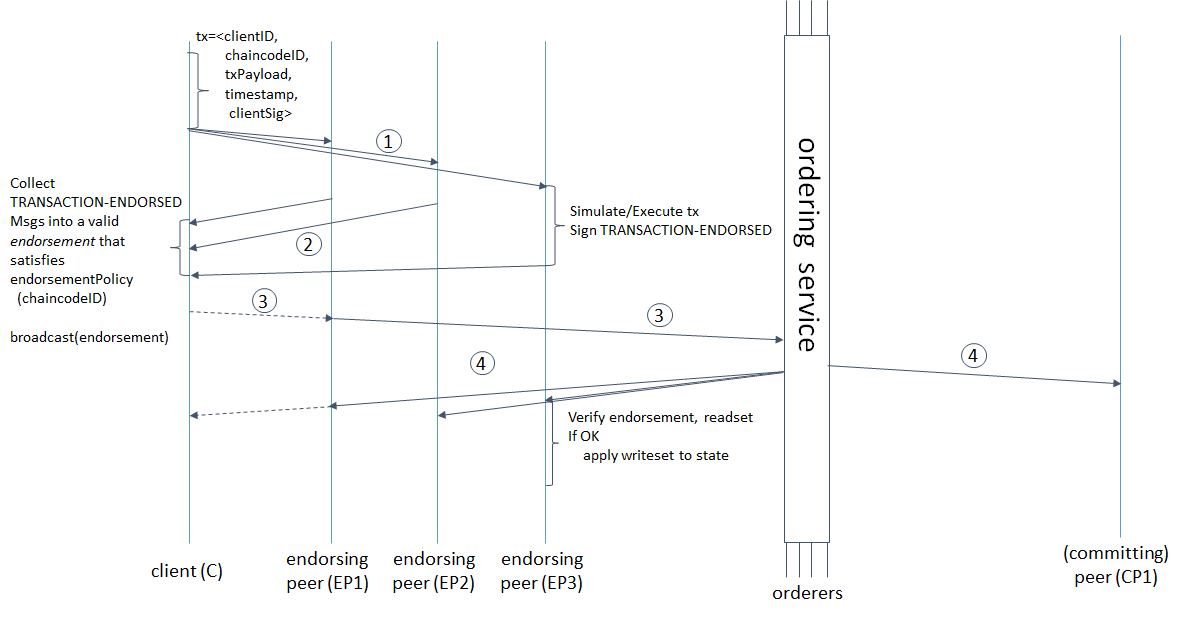
\includegraphics[scale=0.5]{media/fabric_workflow.png}
\caption[Consensus workflow in Hyperledger Fabric]{Consensus workflow in Hyperledger Fabric. Available in~\cite{IBMResearch2017}.}
\label{fig:fabric_workflow}
\end{figure}

Compared to other blockchains, this consensus mechanism has some advantages, though its application is somewhat limited to some use cases. Table~\ref{table:consensus_comparison} summarizes some points of difference between a blockchain using Proof of work and one, like Hyperledger, using a BFT state machine consensus.


%%%%%%%%%%%%%%%% TABELA COMPARATIVA %%%%%%%%%%%%%%%%%%%%%%%%%%

% Please add the following required packages to your document preamble:
% \usepackage[table,xcdraw]{xcolor}
% If you use beamer only pass "xcolor=table" option, i.e. \documentclass[xcolor=table]{beamer}
\begin{table}[]
\centering
\caption{Comparison between traditional PoW consensus and Hyperledger's BFT consensus mechanism}
\label{table:consensus_comparison}
\resizebox{\textwidth}{!}{
\begin{tabular}{c|
>{\columncolor[HTML]{FFCCC9}}c |
>{\columncolor[HTML]{D9FFAB}}c |}
\cline{2-3}
\multicolumn{1}{l|}{}                                                                                                             & \cellcolor[HTML]{ECF4FF}\textbf{\begin{tabular}[c]{@{}c@{}}Proof of Work \\ (Bitcoin, Ethereum, ...)\end{tabular}}                                                         & \cellcolor[HTML]{ECF4FF}\textbf{\begin{tabular}[c]{@{}c@{}}BFT state machine replication \\ (Hyperledger, Ripple, ...)\end{tabular}}                                                          \\ \hline
\multicolumn{1}{|c|}{\cellcolor[HTML]{ECF4FF}\textbf{\begin{tabular}[c]{@{}c@{}}Membership \\ type\end{tabular}}}                 & \cellcolor[HTML]{EFEFEF}{\color[HTML]{000000} Permissionless}                                                                                                              & \cellcolor[HTML]{EFEFEF}{\color[HTML]{000000} Permissioned}                                                                                                                                   \\ \hline
\multicolumn{1}{|c|}{\cellcolor[HTML]{ECF4FF}\textbf{\begin{tabular}[c]{@{}c@{}}User IDs \\ (Sybil attack)\end{tabular}}}         & \cellcolor[HTML]{D9FFAB}{\color[HTML]{000000} \begin{tabular}[c]{@{}c@{}}Decentralized, Anonymous \\ (Decentralized protection by \\ PoW compute/hash power)\end{tabular}} & \cellcolor[HTML]{FFFC9E}{\color[HTML]{000000} \begin{tabular}[c]{@{}c@{}}Centralized, all Nodes know all other \\ Nodes (identity management protects \\ against Sybil attacks)\end{tabular}} \\ \hline
\multicolumn{1}{|c|}{\cellcolor[HTML]{ECF4FF}\textbf{\begin{tabular}[c]{@{}c@{}}Scalability \\ (no. of nodes)\end{tabular}}}      & \cellcolor[HTML]{D9FFAB}{\color[HTML]{000000} Excellent, \textgreater100k nodes}                                                                                           & {\color[HTML]{000000} \begin{tabular}[c]{@{}c@{}}Can scale to 100 nodes, with certain \\ performance degradation\end{tabular}}                                                                \\ \hline
\multicolumn{1}{|c|}{\cellcolor[HTML]{ECF4FF}\textbf{\begin{tabular}[c]{@{}c@{}}Peak \\ Throughput\end{tabular}}}                 & {\color[HTML]{000000} \begin{tabular}[c]{@{}c@{}}from 7tx/sec (Bitcoin) and\\ 15tx/sec (Public Ethereum)\end{tabular}}                                                     & {\color[HTML]{000000} \begin{tabular}[c]{@{}c@{}}\textgreater10k tx/sec with existing \\ implementation in software \\ {[}\textgreater10 nodes{]}\end{tabular}}                               \\ \hline
\multicolumn{1}{|c|}{\cellcolor[HTML]{ECF4FF}\textbf{\begin{tabular}[c]{@{}c@{}}Power \\ efficiency\end{tabular}}}                & {\color[HTML]{000000} \textgreater1 GW (Bitcoin)}                                                                                                                          & {\color[HTML]{000000} Good (commodity hardware)}                                                                                                                                              \\ \hline
\multicolumn{1}{|c|}{\cellcolor[HTML]{ECF4FF}\textbf{\begin{tabular}[c]{@{}c@{}}Temporary\\ forks in \\ blockchain\end{tabular}}} & {\color[HTML]{000000} \begin{tabular}[c]{@{}c@{}}Possible (leads to double-spending\\ attacks)\end{tabular}}                                                               & {\color[HTML]{000000} Not possible}                                                                                                                                                           \\ \hline
\multicolumn{1}{|c|}{\cellcolor[HTML]{ECF4FF}\textbf{\begin{tabular}[c]{@{}c@{}}Consensus \\ Finality\end{tabular}}}              & {\color[HTML]{000000} No}                                                                                                                                                  & {\color[HTML]{000000} Yes}                                                                                                                                                                    \\ \hline
\end{tabular}
}
\end{table}



%%%%%%%%%%%%%%%%%%%%%%%%%%%%%%%%%%%%%%%%%%%%%%%%%%%%%%%%%%%%%%


In brief conclusion, Hyperledger allows for a permissioned blockchain which sacrifices some decentralization for scalability and performance. By using a different consensus mechanism, most of the issues of public blockchains vanish. Furthermore, data access must be authorized, such that sensitive data in a channel is protected, one of the requirements for data in supply chains. Thus, Hyperledger Fabric's features are adequate for SCM's requirements in a way that is difficult to achieve in public blockchains.

\subsection{Hyperledger Composer}
\label{sec:composer-background}
Hyperledger Composer is another tool which works together with Fabric to allow for an easier approach to modeling a blockchain network. It is actually a higher level abstraction of Fabric, which allows for a big reduction in the lines of code written and simplifies the whole process of building a business network and deploying it, as well as the process of managing the identities of the network's participants. The whole documentation for the project is continuously being updated at their website~\cite{LinuxFoundation2018}.

It features a nice and intuitive graphical user interface to manage all of its components, and it also features a REST server to expose the blockchain to outside applications.

\subsubsection{Business Network}

A business network is a model of all the data in the blockchain, which includes all the objects, functions, transactions and identities that will connect to each other and be saved on the ledger. It is basically an abstraction of the chaincode that will be installed onto Fabric. A business network, being a network model, can be deployed into an instance that runs on a certain number of nodes.

Composer features a custom modeling language which makes it easier to define a business network. It is divided into 4 main components, as can be seen in Figure~\ref{fig:composer_abstraction}.

\begin{figure}[h]
\centering
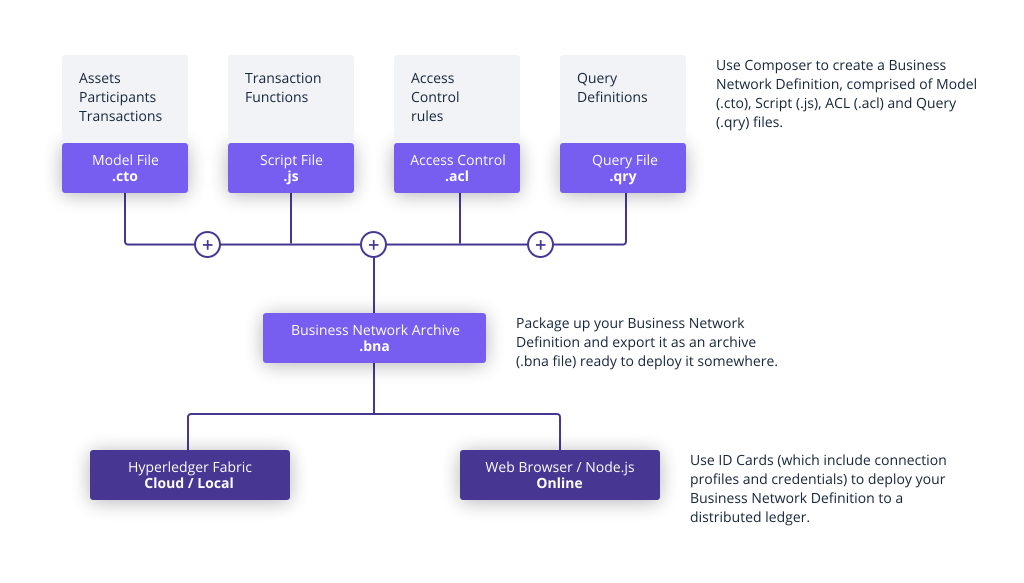
\includegraphics[scale=0.40]{media/Composer-Diagram.png}
\caption[Hyperledger Composer abstraction over Fabric]{Hyperledger Composer abstraction over Fabric. Available in Composer's documents~\cite{ComposerIntro}.}
\label{fig:composer_abstraction}
\end{figure}

If a business network model is deployed multiple times with a different sets of nodes each time, it will simply constitute different instances of a network model. Each instance will constitute a separate network with a separate ledger, independent from the other networks. This is analog to modelling a class in a object oriented programming and then instancing it multiple times. Each instance is separate from the others, even though it is based on the same model. Therefore, a good model design can be used by several businesses separately, and each can configure the model to represent the topology they are looking for.

The 4 main components: 

\paragraph{Model File} This is where all the main data components are defined. \textbf{Assets} are the main "objects" that are handled in transactions, and they can represent a variety of things. One example can be a "car". \textbf{Participants} are the types of people that will be participating in the network. One example participant can be "Customer", which will have fields like "Balance" and "Name". An instance of a participant can be linked to a real identity of a person using the blockchain. \textbf{Transactions} are the most important data object. They model what actions can be taken, and they usually have some data fields associated, which act as the input of the transaction. An example of a transaction can be "BuyCar", which could have as parameters the car ID, and a participant could then call this transaction, if they had the permission to do so. All these 3 components, Assets, Participants and Transactions have their own registry. While the Assets and Participants registries are mutable, the Transactions registry is not. Additionally, another type of object can be defined in this file, \textbf{Events}, which can be emitted by transactions and subscribed by applications which can handle them, for instance, to generate notifications.

\paragraph{Script File} This file contains all the functions that define how a transaction behaves and what kind of data it processes and outputs. It can also have additional auxiliary functions.

\paragraph{Access Control} This is where the access rules are defined. These rules include restrictions on who can invoke which transactions, who can read the data, and many other permissions.

\paragraph{Query File} This file includes some queries that can retrieve information from the blockchain. This information might include any assets, participants or transaction history, and it is also subject to the access control rules. These queries are both exposed to outside applications through the composer REST server and to the Script file functions.

All of these components can be compiled into one file (.bna), which is then deployed onto Fabric.

\subsubsection{Authentication and Identities}

Hyperledger Composer also features identity management. An identity is a digital certificate and private key, in the form of an account which can interact with the blockchain network. Within a certain business network, an identity can even be bound to a certain instance of a Participant type. For example, if there is a participant type called "Customer", an instance of that participant called "Customer1" can be created, which can then be bound to some real person's account. That person will then be able to interact with the blockchain, but will be bound by whatever access rules the participant "Customer" is bound by. 

In order to make identity management easier, Composer has a feature called "Business Network Cards". These cards are files which can are associated with an identity and a network, and also act as a private key. If a user possesses a card, they can import it to prove their identity and start interacting with the blockchain.

\subsubsection{Fabric Topology}

Composer also has configuration files for some of Fabric's properties. It possesses files to determine which organizations exist and which kind of nodes they possess, along with their mapping. It also has a definition for the endorsement policies.


\subsection{Corda}
Corda's take on blockchains vastly differs from Ethereum or Hyperledger. Traditionally, banks have their own ledger, but Corda wants to unify these ledger's into one, claiming that it improves the cost and efficiency. Corda focuses solely on providing a distributed ledger for financial services, where financial agreements can be recorded and managed, available to any financial institution\cite{Brown2016}. 

This is a very specific purpose, which means that Corda's application on Supply Chains would be rather limited, to fixing payments and agreements, perhaps. Even Corda's own smart contracts are pretty limited in what they allow, in comparison to Ethereum's, since they do not allow for all the freedom of computation. In theory, Corda is limited to the financial and legal contracts domain, with the functionality for custom contracts being very limited.

\begin{figure}[h]
\centering
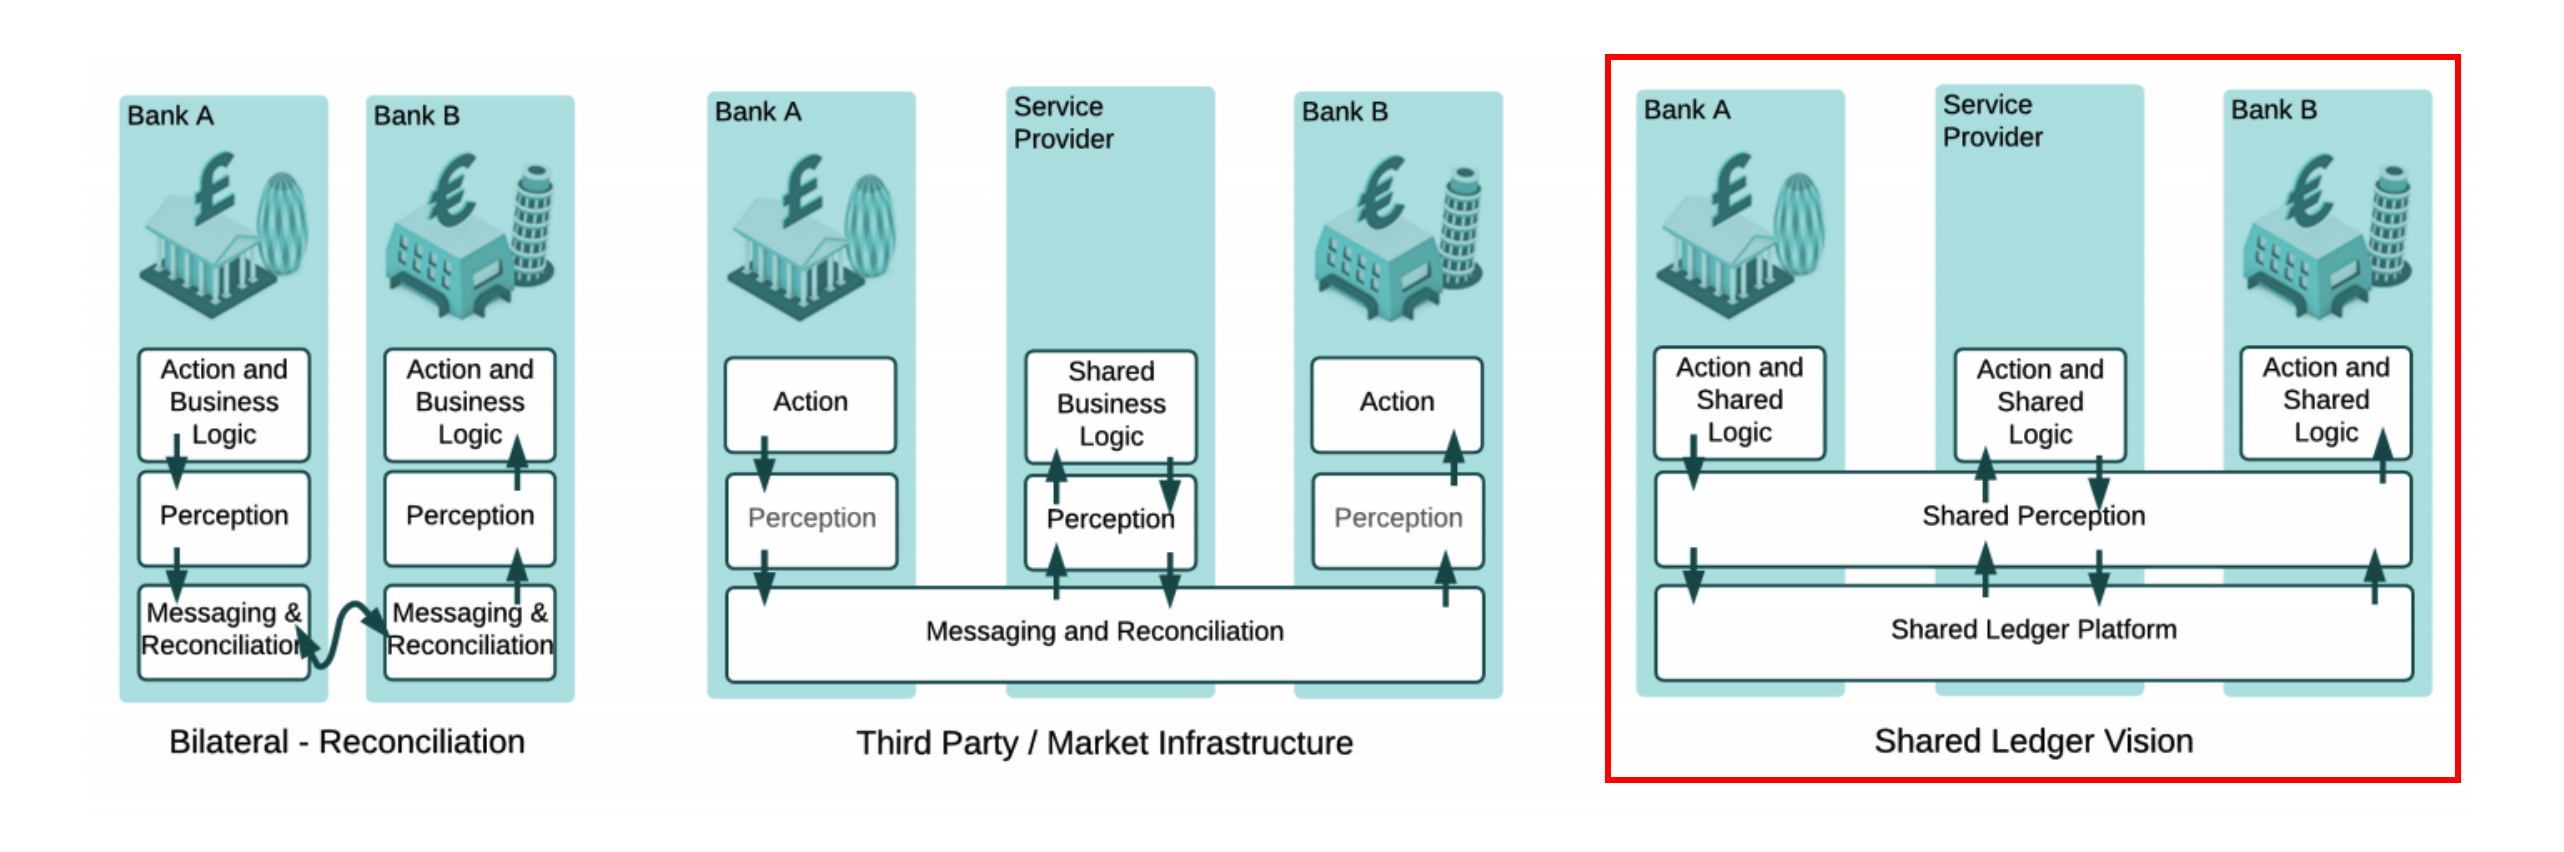
\includegraphics[scale=0.16]{media/corda_shared_ledger.png}
\caption[Corda's vision on a Shared Ledger]{Corda's vision on a Shared Ledger. Available in Corda's White Paper~\cite{Brown2016}.}
\label{fig:shared_ledger}
\end{figure}

\subsection{Concepts}
Corda is also a \textbf{permissioned blockchain}. While the ledger is global, some transactions and agreements involve only certain groups and should be visible only to the participating parties or those with a reason to be able to see them. 

There are some other important concepts to understand how Corda works:
\paragraph{State Objects} The state of the ledger, where the agreements are set and stored, in the code from the contracts.
\paragraph{Transactions} These are the actions that change the state of the ledger.
\paragraph{Transaction Protocols} It is the business logic that enables the coordination of actions, through the smart contract code.


\subsubsection{CorDapps}
CorDapps are distributed applications running on the Corda platform. The concepts of State Objects, Transaction Protocols, among others, all fit into these distributed applications.

The functionality of these applications is, however, rather limited, since a CorDapp's ultimate goal is to program a specific agreement, which will then lead to updates on the ledger. So, similarly to a "smart contract", the execution of CorDapp's leads to transactions which change the state of the ledger, fixing immutable agreements into the blockchain.

These applications have code, just like a smart contract would. But, while a normal smart contract is just code, a program, CorDapps have another side to them: they incorporate legal prose into the code, transforming them into something akin of a "smart legal contract", legally enforceable contracts, clearly designed for the highly regulated environments of the financial industry.

As with Ethereum, Corda also uses a virtual machine. In this case it is the Java Virtual Machine (JVM), and the applications are written in Java.


\subsection{Comparison}
Comparison's between these three platforms are recurrent, though Hyperledger and Corda might have more in common with each other than with Ethereum. 
Valenta~\cite{Valenta2017} concisely describes the main points of difference between these frameworks, with a focus on the consensus process and general characteristics of the frameworks. 

He concluded that Ethereum is more of a general purpose platform, while Fabric tries a different solution, adaptable to a different set of problems. Fabric is flexible and customizable in ways that the other frameworks are not. On the other end, Corda  was designed with one specific application in mind, financial services, and it is rigid in that sense, which actually made its architecture a lot more simple compared to Fabric's. It is also arguable that Hyperledger can be tailored to resemble Corda, due to its modularity, as Corda is not really a competitor of Hyperledger, but rather a complement. 

\paragraph{Hyperledger vs Corda} In one sense, Corda has more of an out-of-the box experience, while with Fabric, the logic would have to be implemented. Composer does make Fabric more user-friendly, but it is still hard to setup and configure, compared to Corda. It all comes down to what kind of system we want to build, and what are its the final objectives, functionalities and requirements.

\paragraph{Ethereum vs Hyperledger} Also, as already pointed out in Section~\ref{hyperledger_architecture}, a permissioned ledger like in Hyperledger might better fit the supply chain industry requirements than Ethereum, though one solution does not discard the other. Another important aspect to distinguish is also the difference in performance between these platforms.



\subsubsection{Performance}
\label{sec-performance-comparison}
The difference in performance of various blockchain platforms is a crucial topic to address, that might lead to choosing one platform over another, with similar functionalities. In the case of Supply Chain, it might be important to measure the difference in performance of Ethereum and Hyperledger, for instance. 

Pongnumkul has conducted a performance analysis of private deployments of these platforms~\cite{Pongnumkul2017} and he reached some interesting conclusions. In summary, \textbf{Hyperledger's performance is higher in every aspect than Ethereum's (on a private deployment)}, but, for the same resources, \textbf{Ethereum can actually handle a higher number of concurrent transactions}. 

The metrics used in the analysis are \textbf{throughput}, \textbf{latency} and \textbf{execution} time.
In every test performed, Hyperledger had a higher throughput, lower latency and lower execution time than Ethereum. The disparity between these numbers also grew with the number of transactions, with Ethereum's performance degrading much more than Hyperledger's for the same increase in transactions. This means that Hyperledger not only performs better, it also scales better, as seen in Figure~\ref{fig:latency_comparison}.

\begin{figure}[h]
\centering
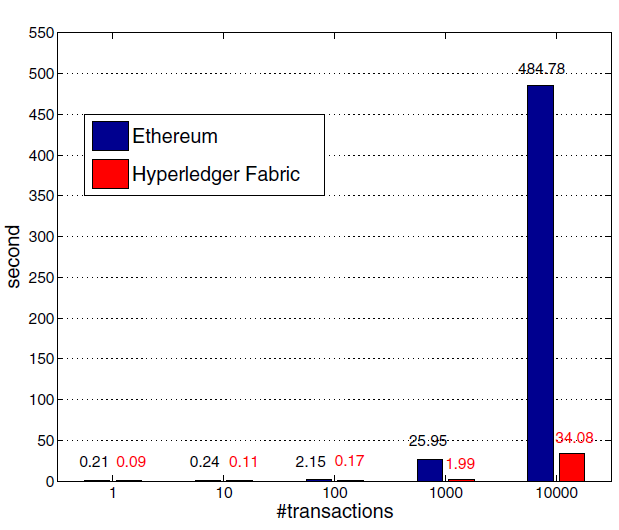
\includegraphics[scale=0.75]{media/average_latency_frameworks.png}
\caption[Comparison of average latency between Ethereum and Hyperledger, with growing number of transactions]{Comparison of average latency between Ethereum and Hyperledger, with growing number of transactions. Available in~\cite{Pongnumkul2017}.}
\label{fig:latency_comparison}
\end{figure}

Another interesting conclusion was that, with a really high number of transactions (10000), Hyperledger only took 3.57 seconds to finish executing the first transaction, while Ethereum took 361.36 seconds, showing that Ethereum's network clogs easily and is slow to start up, while Hyperledger executes the transactions more consistently. This was exactly one of the reasons for the revision in the architecture of Fabric.

%\section{Tendermint}
% Fabric takes a similar approach to Tendermint, but is more opinionated about how the state is managed, and requires that all application behaviour runs in potentially many docker containers, modules it calls “chaincode”. It uses an implementation of PBFT. from a team at IBM that is augmented to handle potentially non-deterministic chaincode It is possible to implement this docker-based behaviour as a ABCI app in Tendermint, though extending Tendermint to handle non-determinism remains for future work.